% ------------------------------------------------------------------------------
% Problem Statement
% ------------------------------------------------------------------------------

\chapter{Problem Statement}\label{chap:problemstatement}

	%O Imageamento em Microondas é um problema inverso de espalhamento eletromagnético. Por ter essa natureza, sua grandezas são definidas em termos das equações de Maxwell as quais descrevem o fenômeno eletromagnético. Particularmente, o problema pode ser escrito em forma de uma equação integral, o que é muito comum para problemas que envolve radiação de uma corrente, seja ela impressa ou induzida. Ao invés de se determinar o efeito a partir de uma causa, o problema é definido de maneira inversa. Por causa disso, existem várias características peculiares para esse tipo problema que é considerado mal-posto na literatura.
	Microwave Imaging is an Electromagnetic Inverse Scattering Problem (EISP). Because of its nature, its magnitudes are defined in terms of Maxwell's equations which describe the electromagnetic phenomenon. In particular, the problem can be written in the form of an integral equation, which is very common for problems involving radiation from a current, whether impressed or induced. Rather than determining the effect from a cause, the problem is defined inversely. Thus, there are several characteristics peculiar to this kind of problem which is considered an ill-posed one in the literature.
	
	%Este capítulo tem por objetivo descrever de uma maneira geral o modelo matemático que representa o problema e discutir importantes aspectos associados. Primeiro, será apresentado a modelagem eletromagnética do problema para que, em seguida, seja desenvolvida a equação que relaciona todas as grandezas importantes para o problema. Posteriormente, alguns fundamentos sobre problemas inversos são apresentados. Logo após, vários aspectos importantes do problema são discutidos. Por fim, é apresentada uma conclusão destacando os principais pontos do capítulos. Também foram escritos os apêndices A, B e C como material de suporte para vários conceitos e deduções que serão utilizados nesse capítulo.
	This chapter aims to describe in a general way the mathematical model which represents the problem and to discuss its most important aspects. In Section \ref{chap:problemstatement:eletromagnetic}, the electromagnetic model will be presented. Then, in Section \ref{chap:problemstatement:integral}, the equation which relates all the required quantities will be developed. Subsequently, some fundamentals about inverse problems are presented in Section \ref{chap:problemstatement:inverse}. Afterward, several important aspects of the problem are discussed in Section \ref{chap:problemstatement:eisp}. Finally, a conclusion is presented highlighting the main topics of the chapter. Appendices \ref{app:green}, \ref{app:integral} and \ref{app:functional} were also written as supporting material for several concepts and deductions that will be used in this chapter.

	\section{Electromagnetic Theory}\label{chap:problemstatement:eletromagnetic}
	
		Maxwell's equations mathematically describe the electromagnetic phenomena. The four equations relate fields and sources in space and time. They are expressed as follows \citep{harrington2001}:
		\begin{eqnarray}
			\nabla\times\boldsymbol{\mathcal{E}}(\mathbf{r}, t) &=& - \frac{\partial\boldsymbol{ \mathcal{B}}}{\partial t}(\mathbf{r}, t) \label{eq:2:maxwell:time:1} \\
			\nabla\times\boldsymbol{\mathcal{H}}(\mathbf{r}, t) &=& \frac{\partial\boldsymbol{ \mathcal{D}}}{\partial t}(\mathbf{r}, t) + \boldsymbol{\mathcal{J}}(\mathbf{r}, t) \label{eq:2:maxwell:time:2} \\
			\nabla\cdot\boldsymbol{\mathcal{D}}(\mathbf{r}, t) &=& \rho(\mathbf{r}, t) \label{eq:2:maxwell:time:3} \\
			\nabla\cdot\boldsymbol{\mathcal{B}}(\mathbf{r}, t) &=& 0 \label{eq:2:maxwell:time:4}
		\end{eqnarray}
	
		The vector $\mathbf{r} = x\mathbf{x} + y\mathbf{y} + z\mathbf{z} = \langle x, y, z \rangle$ denotes the space coordinates (in meters [m])  and $t$ is the time (in seconds [s]). The vectors $\boldsymbol{\mathcal{E}}$, $\boldsymbol{\mathcal{H}}$, $\boldsymbol{\mathcal{D}}$, and $\boldsymbol{\mathcal{B}}$ represent electric field intensity (in volts per meter [V/m]), magnetic field intensity (in amperes per meter [A/m]), electric flux density (in coulombs per square meter [C/m$^2$]), and magnetic flux density (in tesla [T]). The sources are the electric current density $\boldsymbol{\mathcal{J}}$ (in amperes per square meter [A/m$^2$]) and the volume electric charge density $\rho$ (in coulombs per cubic meter [C/m$^3$]).
	
		Maxwell's equations can also be written in harmonic form, i.e., when time dependence is expressed in cosinusoidal form. In this case, the fields and sources can be written as quantities of a complex nature based on the following relationship:
		\begin{equation}
			\boldsymbol{\mathcal{F}}(\mathbf{r}, t) = \mathfrak{Re}\{\mathbf{F}(\mathbf{r})e^{j\omega t}\} \label{eq:2:fourier}
		\end{equation}
	
		In this way, the real vector field $\boldsymbol{\mathcal {F}}$ is completely described by the complex field $\mathbf{F}$ and the known angular frequency $\omega = 2\pi f$ (in radians per second [rad/s]). In \eqref{eq:2:fourier}, $j=\sqrt{-1}$ is the imaginary unit. Thus, Maxwell's equations in harmonic regime are defined as:
		\begin{eqnarray}
			\nabla\times\mathbf{E}(\mathbf{r}) &=& - j\omega\mathbf{B}(\mathbf{r}) \label{eq:2:maxwell:har:1} \\
			\nabla\times\mathbf{H}(\mathbf{r}) &=&  j\omega\mathbf{D}(\mathbf{r}) + \mathbf{J}(\mathbf{r}) \label{eq:2:maxwell:har:2} \\
			\nabla\cdot\mathbf{D}(\mathbf{r}) &=& \rho(\mathbf{r}) \label{eq:2:maxwell:har:3} \\
			\nabla\cdot\mathbf{B}(\mathbf{r}) &=& 0 \label{eq:2:maxwell:har:4}
		\end{eqnarray}
	
		In addition to Maxwell's equations, constitutive relationships are important for describing the relationship between fields and the environments in which they exist. In general, the relationships between field intensity and flux density vectors are expressed as:
		\begin{eqnarray}
			\mathbf{D}(\mathbf{r}) &=& F_1(\mathbf{E}, \mathbf{H})(\mathbf{r}) \label{eq:2:constitutive:general:1} \\
			\mathbf{B}(\mathbf{r}) &=& F_2(\mathbf{E}, \mathbf{H})(\mathbf{r}) \label{eq:2:constitutive:general:2}
		\end{eqnarray}
	
		The operators $F_1$ and $F_2$ represent the relationships between these two types of vector quantities. They are defined according to the medium in which these fields are present. Depending on the properties of each medium, these operators can be: linear or nonlinear; dependent on $\mathbf{E}$ and $\mathbf{H}$ or just one of these two vectors; defined as tensors or even scalars. Considering only linear, isotropic, and non-dispersive media, the constitutive relationships can be simplified to:
		\begin{eqnarray}
			\mathbf{D}(\mathbf{r}) &=& \epsilon_0\epsilon_r(\mathbf{r})\mathbf{E}(\mathbf{r}) \label{eq:2:constitutive:liniso:1} \\
			\mathbf{B}(\mathbf{r}) &=& \mu_0\mu_r(\mathbf{r})\mathbf{H}(\mathbf{r}) \label{eq:2:constitutive:liniso:2}
		\end{eqnarray}
	
		The constants $\epsilon_0$ and $\mu_0$ represent vacuum dielectric permittivity (in farads per meter [F/m]) and vacuum magnetic permeability (in henries per meter [H/m]), respectively. These constants are already known and are equivalent to $\epsilon_0\approx 8.854\times10^{-12}$ [F/m] and $\mu_0 = 4\pi\times10^{-7}$ [H/m]. The dimensionless quantities $\epsilon_r$ and $\mu_r$ represent the relative dielectric permittivity and magnetic permeability, i.e., they define the electromagnetic properties of a medium in proportion to the vacuum ones. They can be defined as functions which map their scalar value in space, either to delimit objects or to represent heterogeneities. In addition to these properties, if conductive objects are considered, the source $\mathbf{J}$ in \eqref{eq:2:maxwell:har:2} must be rewritten as the sum of an impressed current $\mathbf{J}_i $ and an induced one $\sigma\mathbf{E}$ defined by Ohm's law, i.e., $\mathbf{J}(\mathbf {r}) = \mathbf{J}_i (\mathbf{r}) + \sigma(\mathbf{r})\mathbf{E}(\mathbf{r})$. The electrical conductivity $\sigma$ (in siemens per meter [S/m]) is the property that describes the ability of the medium to induce current in the presence of an electric field. From this definition, \eqref{eq:2:maxwell:har:2} can be rewritten as:
		\begin{eqnarray}
			\nabla\times\mathbf{H}(\mathbf{r}) &=&  j\omega\epsilon_0\epsilon_r\mathbf{E}(\mathbf{r}) + \sigma(\mathbf{r})\mathbf{E}(\mathbf{r})+ \mathbf{J}_i(\mathbf{r}) \label{eq:2:complexmedia:1} \\
			 &=&  j\omega\epsilon_0\left(\epsilon_r(\mathbf{r}) -j\frac{\sigma(\mathbf{r})}{\omega\epsilon_0}\right)\mathbf{E}(\mathbf{r}) +  \mathbf{J}_i(\mathbf{r}) \label{eq:2:complexmedia:2} \\
			&=&  j\omega\epsilon(\mathbf{r})\mathbf{E}(\mathbf{r}) +  \mathbf{J}_i(\mathbf{r}) \label{eq:2:complexmedia:3}
		\end{eqnarray}
	
		The quantity $\epsilon = \epsilon_0\epsilon_r - j\sigma/\omega$ is called effective dielectric permittivity and is a complex scalar.
	
	\section{Integral Equations}\label{chap:problemstatement:integral}
	
		The scattering problem consists of a source $\mathbf{J}_i(\mathbf{r})$ which propagates a wave through a medium with electromagnetic properties $\epsilon_b$ and $\mu_b$ and in the presence of a non-homogeneous scatter with properties $\epsilon(\mathbf{r})$ and $\mu(\mathbf{r})$ (Figure \ref{fig:2:scattering}) \citep{chew1995}. In this scenario, the equations \eqref{eq:2:maxwell:har:1}-\eqref{eq:2:maxwell:har:4} are valid for any point $\mathbf{r}$ of space. With the aid of \eqref{eq:2:constitutive:liniso:2}, the equation \eqref{eq:2:maxwell:har:1} can be rewritten as:
		\begin{eqnarray}
				\nabla\times\mathbf{E}(\mathbf{r}) &=& - j\omega\mu(\mathbf{r})\mathbf{H}(\mathbf{r}) \label{eq:2:waveequations:1} \\
				\mu^{-1}(\mathbf{r})\nabla\times\mathbf{E}(\mathbf{r}) &=& - j\omega\mathbf{H}(\mathbf{r}) \label{eq:2:waveequations:2} 
		\end{eqnarray}
	
	    \begin{figure}[!tb]
			\centering
			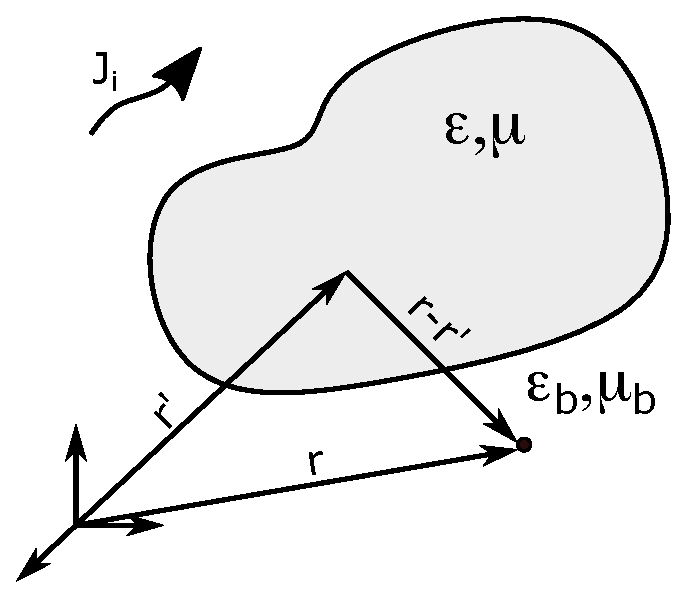
\includegraphics[width=0.5\textwidth]{./figuras/scattering}
			\caption{General scattering problem.}
			\label{fig:2:scattering}
		\end{figure}
	
		If we take the curl of \eqref{eq:2:waveequations:2}, we can use \eqref{eq:2:complexmedia:3} to obtain an equation with only the electric field:
		\begin{eqnarray}
			\nabla\times\mu^{-1}(\mathbf{r})\nabla\times\mathbf{E}(\mathbf{r}) &=& - j\omega\nabla\times\mathbf{H}(\mathbf{r}) \label{eq:2:waveequations:3} \\ \nabla\times\mu^{-1}(\mathbf{r})\nabla\times\mathbf{E}(\mathbf{r}) &=& - j\omega\left(j\omega\epsilon(\mathbf{r})\mathbf{E}(\mathbf{r}) +  \mathbf{J}_i(\mathbf{r})\right) \label{eq:2:waveequations:4}
		\end{eqnarray}
	
		Through this, we obtain the vector wave equation:
		\begin{equation}
					\nabla\times\mu^{-1}(\mathbf{r})\nabla\times\mathbf{E}(\mathbf{r}) - \omega^2\epsilon(\mathbf{r})\mathbf{E}(\mathbf{r})  = - j\omega\mathbf{J}_i(\mathbf{r}) \label{eq:2:waveequations:5} 
		\end{equation}
	
		Subtracting both sides of \eqref{eq:2:waveequations:5} by $\nabla\times\mu_b^{-1}\nabla\times\mathbf{E}(\mathbf{r})-\omega^2\epsilon_b\mathbf{E}(\mathbf{r})$, one can obtain:
		\begin{multline}
			\nabla\times\left(\mu^{-1}(\mathbf{r})-\mu_b^{-1}\right)\nabla\times\mathbf{E}(\mathbf{r}) - \omega^2\left(\epsilon(\mathbf{r})-\epsilon_b\right)\mathbf{E}(\mathbf{r}) \\ =  -  j\omega\mathbf{J}_i(\mathbf{r}) -\nabla\times\mu_b^{-1}\nabla\times\mathbf{E}(\mathbf{r}) + \omega^2\epsilon_b\mathbf{E}(\mathbf{r}) \label{eq:2:waveequations:6}
		\end{multline}
		\begin{multline}
			\nabla\times\mu_b^{-1}\nabla\times\mathbf{E}(\mathbf{r}) - \omega^2\epsilon_b\mathbf{E}(\mathbf{r}) \\ = -j\omega\mathbf{J}_i(\mathbf{r}) + \omega^2\left(\epsilon(\mathbf{r})-\epsilon_b\right)\mathbf{E}(\mathbf{r}) -	\nabla\times\left(\mu^{-1}(\mathbf{r})-\mu_b^{-1}\right)\nabla\times\mathbf{E}(\mathbf{r}) \label{eq:2:waveequations:7} 
		\end{multline}
	
		The right side of \eqref{eq:2:waveequations:7} represents the effective current source $\mathbf{J}$. This equation is analogous to the problem described in \autoref{app:integral}. Therefore, similarly to \eqref{eq:app:integral:final}, the solution of \eqref{eq:2:waveequations:7} is:
		\begin{multline}
			\mathbf{E}(\mathbf{r}) =  j\omega \int_V d\mathbf{r^\prime}~ \mathbf{\bar{G}}(\mathbf{r},\mathbf{r^\prime})\cdot\mu_b\mathbf{J}(\mathbf{r}) + \omega^2\int_V d\mathbf{r^\prime}~\mathbf{\bar{G}}(\mathbf{r},\mathbf{r^\prime})\cdot\mu_b\left(\epsilon(\mathbf{r^\prime})-\epsilon_b\right)\mathbf{E}(\mathbf{r^\prime}) \\ - \int_V d\mathbf{r^\prime}~\mathbf{\bar{G}}(\mathbf{r},\mathbf{r^\prime})\cdot\mu_b\nabla^\prime\times\left(\mu^{-1}(\mathbf{r^\prime})-\mu_b^{-1}\right)\nabla^\prime\times\mathbf{E}(\mathbf{r^\prime}) \label{eq:2:waveequations:8}
		\end{multline}
	
		The first term on the right side of \eqref{eq:2:waveequations:8} is the field produced by the impressed source of the problem, which is also called the incident field $\mathbf{E}_i(\mathbf{r})$. The function $\mathbf{\bar{G}}(\mathbf{r},\mathbf{r^\prime})$ is the Dyadic Green's Function for homogeneous medium \eqref{eq:app:green:17} and it is the impulse response, i.e., the solution of the equations for a point source (see Appendix \ref{app:green} for further information). The second term represents the field due to the displacement or conduction electric currents, while the third term represents the field due to the magnetic polarization charges. If we suppose that there are only non-magnetic materials, i.e., $\mu = \mu_b = \mu_0$, then we can rewrite \eqref{eq:2:waveequations:8} as:
		\begin{equation}
			\mathbf{E}(\mathbf{r}) = \mathbf{E}_i(\mathbf{r}) + k_b^2\int_V d\mathbf{r^\prime}~\mathbf{\bar{G}}(\mathbf{r},\mathbf{r^\prime})\cdot\chi(\mathbf{r^\prime})\mathbf{E}(\mathbf{r^\prime}) \label{eq:2:waveequations:final}
		\end{equation}
	
		\noindent in which:
		\begin{equation}
			\chi(\mathbf{r}) = \frac{\epsilon_r(\mathbf{r})}{\epsilon_{rb}}-1-j\frac{\sigma(\mathbf{r})-\sigma_b}{\omega\epsilon_b} \label{eq:2:contrast}
		\end{equation}
	
		\noindent is called the contrast function and $k_b = \omega\sqrt{\mu_0\epsilon_b}$ is the background wavenumber (in meters [m]).
	
	\section{Basic Theory of Inverse Ill-Posed Problems}\label{chap:problemstatement:inverse}
	
		%Para um dado fenômeno nós conhecemos a causa e procuramos conhecer o efeito, estamos lidando com um problema direto. Por um outro lado, se conhecemos o efeito e procuramos a causa, estamos lidando com um problema inverso. Alternativamente, existem outras maneiras de se definir um problema inverso. Conforme definiu \cite{keller1976inverse}, dois problemas são inversos entre si se a formulação de cada uma envolve a solução completa da outra. Além disso, conforme afirmado também por \cite{bertero2020introduction}, no passado, os problemas diretos foram amplamente estudados enquanto os inversos não eram e eram pouco entendidos. Com frequência, os problemas inversos eram também mal-postos.
		There is no rigorous mathematical definition of inverse problems. In fact, when someone defines a problem as the inverse counterpart of some other, this is usually arbitrary. A very known definition was written by \cite{keller1976inverse} in which two problems are inverse to each other if the formulation of each involves the complete solution of the other. Also, as stated by \cite{bertero2020introduction}, the direct problem used to be the one that had been extensively studied while the inverse counterpart used to be one that was still poorly understood. From a physical perspective, for a given phenomenon, if the cause is known and we attempt to know the effect, then we are dealing with a direct or forward problem. On the other hand, if the effect is known and the cause is sought, then we are dealing with an inverse problem.
	
		%\cite{hadamard1923lectures} definiu que um modelo matemático para um problema físico seria bem-posto ou propriamente posto se três condições fossem garantidas. De uma forma matemática, sendo $X$ e $Y$ espaços normais e $\mathcal{K}$ um operador linear ou não no qual $\mathcal{K} : X \rightarrow Y$, a equação $\mathcal{K}\{x\}=y$ é bem-posta se \citep{kirsch2011introduction}:
		One of the reasons for inverse problems being the least attractive one is that they are often ill-posed. \cite{hadamard1923lectures} defined that a mathematical model for a physical problem would be well-posed or properly posed if three conditions were guaranteed. Mathematically, let $X$ and $Y$ be normed spaces and $\mathcal{K}$ a linear or nonlinear operator in which $\mathcal{K} : X \rightarrow Y$, the equation $\mathcal{K}\{x\}=y$ is well-posed if \citep{kirsch2011introduction}:
		\begin{enumerate}
			%\item \textbf{Existência}: para cada $y\in Y$ existe pelo menos um $x\in X$ no qual $\mathcal{K}\{x\}=y$;
			\item \textbf{Existence}: for each $y\in Y$ there is at least one $x\in X$ in which $\mathcal{K}\{x\}=y$;
			%\item \textbf{Unicidade}: para cada $y\in Y$ existe no máximo um $x\in X$ no qual $\mathcal{K}\{x\}=y$;
			\item \textbf{Uniqueness}: for each $y\in Y$ there is at most one $x\in X$ in which $\mathcal{K}\{x\}=y$;
			%\item \textbf{Estabilidade}: a solução $x$ tem dependência contínua em relação a $y$, i.e., para cada sequência $(x_n)\subset X$ no qual $\mathcal{K}\{x_n\}\rightarrow \mathcal{K}\{x\}$ quando $n\rightarrow\infty$, segue-se $x_n\rightarrow x$ quando $n\rightarrow\infty$.
			\item \textbf{Stability}: solution $x$ has continuous dependence on $y$, i.e., for each sequence $(x_n)\subset X$ in which $\mathcal{K}\{x_n\}\rightarrow \mathcal{K}\{x\}$ when  $n\rightarrow\infty$, follows $x_n\rightarrow x$ when $n\rightarrow\infty$ .
		\end{enumerate}
	
		%Quando um problema não atende pelo menos uma dessas condições, então ele é chamado de mal-posto ou impropriamente posto. Entretanto, quando alguma delas é violada, é possível adotar algumas estratégias para que a posição do problema seja corrigida. Por exemplo, quando não existe solução, o espaço de soluções pode ser alargado para que o respectivo critério seja atendido. Quando há muitas soluções, então pode estar faltando alguma informação que restrinja o espaço e garanta a unicidade de solução. No entanto, quando o problema não é estável, então é praticamente impossível encontrar a solução a menos que novas informações sobre ela sejam adicionadas. Conforme afirmado por \cite{lanczos1961linear}, quando se falta informação, não existe artifiício matemático que possa consertar.
		When a problem does not satisfy at least one of these conditions, then it is called ill-posed or improperly posed. However, when any of them is violated, it is possible to adopt some strategies so that the posedness conditions are fulfilled. For example, when there is no solution, the space of solutions can be enlarged so that the respective criterion is satisfied. When there are many solutions, then there may be a lack of information which could reduce space and ensures uniqueness. However, when the problem is not stable, then it is practically impossible to find a solution unless a new information about its form is added. As stated by \cite{lanczos1961linear}, when information is lacking, there is no mathematical trickery that can fix it.
	
		%Além disso, as condições de existência e de unicidade dependem somente da natureza dos espaços e dos operadores. Já a condição de estabilidade depende também da topologia dos espaços, i.e., se o operador inverso $\mathcal{K}^{-1}:X\rightarrow Y$ é contínuo. Essas características estão relacionadas entre si, por exemplo, um operador inverso $\mathcal{K}^{-1}$ é automaticamente contínuo se $\mathcal{K}$ é linear e contínuo e $X$ e $Y$ são espaços de Banach\footnote{Um espaço normal $X$ sobre $\mathbb{R}$ ou $\mathbb{C}$ é chamado completo ou de Banach se toda sequência de Cauchy converge em $X$.}. Ademais, se $\mathcal{K}$ é um operador contínuo e compacto, o problema inverso é mal-posto a não ser que $X$ tenha dimensão finita \citep{colton2019inverse}.
		Besides, the conditions of existence and uniqueness depend only on the nature of the spaces and the operators. The stability condition also depends on whether the operator $\mathcal{K}:X\rightarrow Y$ is surjective. Continuity of the inverse operator $\mathcal{K}^{-1}:Y\rightarrow X$ is also relevant information. For example, an inverse operator $\mathcal{K}^{-1}$ is automatically continuous if $\mathcal{K}$ is linear and continuous and $X$ and $Y$ are Banach spaces (\autoref{def:app:functional:5}). Furthermore, if $\mathcal{K}$ is a continuous and compact operator, the inverse problem is ill-posed unless $X$ is of finite dimension \citep{colton2019inverse}.
		
		%A adição de informações para resolver problemas mal-postos pode ser alcançadas através de estratégias de regularização. Em problemas onde $X$ e $Y$ são espaços de Hilbert\footnote{Um espaço pré-Hilbert é um espaço com um produto interno definido. Um espaço de Hilbert é um espaço pré-Hilbert completo.}, $\mathcal{K}$ é um operador que é linear, compacto\footnote{Um conjunto relativamente compacto é aquele no qual cada sequência tem um ponto de acumulação. Um operador é denominado compacto se mapeia cada conjunto limitado em um conjunto relativamente compacto.} e um-pra-um\footnote{Um operador um-pra-um é aquele que injetivo e surjetivo, i.e., tem solução e única.}; e $y\in Y$ não é conhecido senão por um erro $\delta>0$ tal que:
		The addition of information to solve ill-posed problems can be achieved through regularization strategies. In problems where $X$ and $Y$ are Hilbert spaces, $\mathcal{K}$ is an operator that is linear, compact\footnote{In few words, the compactness of an operator means that its has infinitely small singular values accumulating at zero. A more precise definition is available at \autoref{def:app:functional:7}.}, and one-to-one; and $y\in Y$ is not known except for an error $\delta>0$ such that:
		\begin{equation}
			||y-y^\delta|| \le \delta \label{eq:2:inverse:1}
		\end{equation} 
	
		% \noindent no qual $y^\delta\in Y$. A equação $\mathcal{K}\{x^\delta\}=y^\delta$ geralmente não tem solução, uma vez que $y^\delta$ não está no intervalo $\mathcal{K}(X)$ de $X$. Então, o objetivo seria determinar uma solução $x^\delta\in X$ que se aproxima de $x\in X$. Além disso, é necessário que $x^\delta$ tenha dependência contínua em relação aos dados $y^\delta$. Portanto, o objetivo é contrauir um operador $\mathcal{R}_\alpha : Y \rightarrow X$ linear e limitado que seja uma aproximação de $\mathcal{K}^{-1}$, i.e.:
		\noindent where $y^\delta\in Y$.
		
		The equation $\mathcal{K}\{x^\delta\}=y^\delta$ usually has no solution since $y^\delta$ is not in the range $\mathcal{K}(X)$ of $X$. So, the goal would be to determine a solution  $x^\delta\in X$ that approximates $x\in X$. In addition, $x^\delta$ must depend continuously on the data $y^\delta$. Therefore, the objective is to construct a linear and bounded operator $\mathcal{R}_\alpha : Y \rightarrow X$ that is an approximation of $\mathcal{K}^{-1}$, i.e.:
		\begin{equation}
			\lim\limits_{\alpha\rightarrow0} \mathcal{R}_\alpha\{y\} = x,~\forall x \in X \label{eq:2:inverse:2}
		\end{equation}
	
		%Em outras palavras, o operador $\mathcal{R}_\alpha$ é tal que converge ponto-a-ponto para um operador identidade. Através dessa definição, $x^{\alpha, \delta} = \mathcal{R}_\alpha\{y^\delta\}$ é uma aproximação para a solução $x$ de $\mathcal{K}\{x\}=y$. Uma discussão mais profunda pode ser encontrados em livros sobre análise funcional e regularizadores \citep{kirsch2011introduction,lebedev1996functional}.
		In other words, the $\mathcal{R}_\alpha\{\mathcal{K}\{\cdot\}\}$ operation is such that it converges pointwise to an identity operator. Through this definition, $x^{\alpha, \delta} = \mathcal{R}_\alpha\{y^\delta\}$ is an approximation to the solution $x$ of $\mathcal{K}\{x\}=y$. A more in-depth discussion can be found in books on functional analysis and regularization strategies \citep{kirsch2011introduction,lebedev1996functional}.
	
	\section{The Eletromagnetic Inverse Scattering Problem}\label{chap:problemstatement:eisp}
	
		%Até aqui foram apresentadas os fundamentos para o problema inverso de espalhamento eletromagnético. Esta seção apresenta define o problema apresentando várias formulações possíveis, tanto na representação geral tridimensional quanto num caso particular bidimensional do modo tranversal magnético. Além disso, discussões sobre importantes aspectos do problema são elaboradas, tais como os espaços vetoriais das funções, unicidades, estabilidade, não-linearidade e graus de liberdade.
		So far, the fundamentals for EISP have been introduced. This section presents the problem by describing several possible formulations, both in the general three-dimensional representation and in a particular two-dimensional case (Transverse Magnetic mode). In addition, discussions about important aspects of the problem are elaborated, such as the vector spaces of functions, uniqueness, stability, non-linearity, and degrees of freedom.
	
		\subsection{Formulations}\label{chap:problemstatement:eisp:1}
			%A equação descreve o campo elétrico total observado em ponto através da soma de uma componente incidente e uma outra componente causada as correntes de indução. A esta última componente, denominamos de campo espalhado $\mathbf{E}_s$. Ou seja, a \eqref{eq:2:waveequations:final} pode ser reescrita como:
			The equation \eqref{eq:2:waveequations:final} describes the total electric field through the sum of an incident component and another one caused by induced currents. This latter component is called the scattered field $\mathbf{E}_s$. Particularly, \eqref{eq:2:waveequations:final} can be rewritten as:
			\begin{equation}
				\mathbf{E}(\mathbf{r}) = \mathbf{E}_i(\mathbf{r}) + \mathbf{E}_s(\mathbf{r}) \label{eq:2:eisp:1}
			\end{equation}
	
			\noindent where:
			\begin{equation}
				\mathbf{E}_s(\mathbf{r}) = k_b^2\int_V d\mathbf{r^\prime}~\mathbf{\bar{G}}(\mathbf{r},\mathbf{r^\prime})\cdot\chi(\mathbf{r^\prime})\mathbf{E}(\mathbf{r^\prime}) \label{eq:2:eisp:2}
			\end{equation}
		
			%Quando a função contraste $\chi$ e o campo incidente $\mathbf{E}_i$ são conhecidos dentro de uma região $V$,  o campo total $\mathbf{E}$ pode ser determinado através da equação \eqref{eq:2:waveequations:final}. Este problema é chamado de problema direto. Por um outro lado, se o campo espalhado $\mathbf{E}_s$ é conhecido em um ou um conjunto de pontos $\mathbf{r}$, geralmente fora de $V$, a equação \eqref{eq:2:eisp:2} pode ser utilizada para determinar-se $\chi$. A este problema denominamos de problema inverso de espalhamento (EISP). No entanto, é necessário observar que o campo total na região $V$ também é desconhecido e depende de $\chi$. Desta forma, EISP é um problema não-linear.
			When the contrast function $\chi$ and the incident field $\mathbf{E}_i$ are known within a region $V$, the total field $\mathbf{E}$ can be determined using equation \eqref{eq:2:waveequations:final}. This problem is called the forward or direct problem and the equation \eqref{eq:2:waveequations:final} is an example of a Fredholm Integral Equation of Second Kind \citep{polyanin2008handbook}. On the other hand, if the scattered field $\mathbf{E}_s$ is known at one or a set of points $\mathbf{r}$, usually outside $V$, equation \eqref{eq:2:eisp:2} can be used to determine $\chi$. We call this problem the Electromagnetic Inverse Scattering Problem (EISP). However, it is necessary to note that the total field in $V$ is also unknown and depends on $\chi$. Thus, EISP is a non-linear problem.
			
			%Em EISPs, a equação \eqref{eq:2:eisp:2} é chamada de equação de dados, uma vez que relaciona os dados do problema ($\mathbf{E}_s$) com as variáveis desconhecidas ($\chi$ e $\mathbf{E}$). Ela pode ser escrita na forma de um operador não-linear:
			In EISPs, equation \eqref{eq:2:eisp:2} is called data equation, since it relates the problem data ($\mathbf{E}_s$) with the unknown variables  ($\chi$ and $\mathbf{E}$). This equation belongs to a class called Lippman-Schwinger integral equations \citep{lippmann1950variational}. It can be written in the form of a non-linear operator:
			\begin{equation}
				\mathbf{E}_s(\mathbf{r}) = \mathcal{L}^D\left\{\chi(\mathbf{r^\prime}), \mathbf{E}(\mathbf{r^\prime})\right\},~\mathbf{r}\notin V,~ \mathbf{r^\prime}\in V \label{eq:2:eisp:3}
			\end{equation}
			
			%A equação \eqref{eq:2:waveequations:final} também é utilizada em EISPs e é conhecida como equação de estados. Ela é uma relação entre as variáveis desconhecidas ($\chi$ e $\mathbf{E}$) com uma conhecida a qual é uma entrada geral para o problema ($\mathbf{E}_i$). Também é possível escrever \eqref{eq:2:waveequations:final} em termos de um operador:
			The equation \eqref{eq:2:waveequations:final} is also used in EISPs and is known as the state equation. It is a relationship between unknown variables ($\chi$ and $\mathbf{E}$) with a known one which is a general entry for the problem ($\mathbf{E}_i$). It is also possible to write \eqref{eq:2:waveequations:final}  in terms of an operator:
			\begin{equation}
				\mathbf{E}_i(\mathbf{r}) = \mathbf{E}(\mathbf{r}) - \mathcal{L}^S\left\{\chi(\mathbf{r}), \mathbf{E}(\mathbf{r})\right\}, \mathbf{r}\in V \label{eq:2:eisp:4}
			\end{equation}
		
			%Assim como $\mathcal{L}^D$, $\mathcal{L}^S : U, W \rightarrow W$. Geralmente, esta equação é utilizada em situações onde $\mathbf{r}\in V$, i.e., o operador $\mathcal{L}^D$ pode envolver singularidades. No entanto, existem formas de abordar singularidades nessa equação (confira a seção \ref{app:green:2} do \autoref{app:green}).
			Frequently, this equation is used in situations where $\mathbf{r}\in V$, i.e., the $\mathcal{L}^S$ operator can involve singularities. However, there are approaches to address singularities in this equation (see \autoref{app:green} section \ref{app:green:2}).
			
			%Alternativamente, também é muito encontrado na literatura a formulação do EISP em termos da fonte de contraste $\mathbf{J}_{eq}(\mathbf{r}) = \chi(\mathbf{r})\mathbf{E}(\mathbf{r})$:
			Alternatively, the EISP formulation in terms of the contrast source $\mathbf{J}_{eq}(\mathbf{r}) = \chi(\mathbf{r})\mathbf{E}(\mathbf{r})$ is also widely found in the literature \cite{berg1997constrast}:
			\begin{eqnarray}
				\mathbf{E}_s(\mathbf{r}) &=& k_b^2\int_V d\mathbf{r^\prime}~\mathbf{\bar{G}}(\mathbf{r},\mathbf{r^\prime})\cdot\mathbf{J}_{eq}(\mathbf{r^\prime}) \label{eq:2:eisp:5} \\
				\chi(\mathbf{r})\mathbf{E}_i(\mathbf{r}) &=& \mathbf{J}_{eq}(\mathbf{r}) - k_b^2\chi(\mathbf{r})\int_V d\mathbf{r^\prime}~\mathbf{\bar{G}}(\mathbf{r},\mathbf{r^\prime})\cdot\mathbf{J}_{eq}(\mathbf{r^\prime}) \label{eq:2:eisp:6}
			\end{eqnarray}
		
			%A vantagem desse tipo de formulação é os operadores $\mathcal{L}^D$ e $\mathcal{L}^S$ são lineares. No entanto, ainda existem duas variáveis desconhecidas no problema ($\chi$ e $\mathbf{J}_{eq}$) as quais estão relacionadas de maneira não-linear na \eqref{eq:2:eisp:6}.
			The advantage of this type of formulation is that the $\mathcal{L}^D$ and $\mathcal{L}^S$ operators are linear. However, there are still two unknown variables in the problem ($\chi$ and $\mathbf{J}_{eq}$) that are related in a non-linear fashion in \eqref{eq:2:eisp:6}.
	
			%Também podemos destarcar formas alternativas de se escrever as integrais presentes em \eqref{eq:2:waveequations:final} e \eqref{eq:2:eisp:2} a partir de manipulações com os operadores presentes da função diádica de Green. Esses tipos de manipulações podem ser úteis para facilitar a implementação computacional das equações integrais. Uma manipulação muito comum é mover um dos operadores $\nabla$ dentro da função de Green para fora da integral. A vantagem desse tipo de técnica é reduzir o erro numérico de quadratura. Conforme mostrado na seção 4.4.1 de \citep{chew2009}, se considerarmos a equação \eqref{eq:app:green:12}, a qual representa as integrais em \eqref{eq:2:waveequations:final} e \eqref{eq:2:eisp:2}, a integral pode ser reescrita como:
			There are alternative forms of writing the integrals in \eqref{eq:2:waveequations:final} and \eqref{eq:2:eisp:2} through manipulating the derivative operators of dyadic Green's function. These kinds of manipulations can be convenient to facilitate the computational implementation of integral equations. A very common manipulator is to move one of the $\nabla$ operators within Green's function to the integral. The advantage of this technique is that it reduces the numerical quadrature error. As stated in section 4.4.1 of \cite{chew2009}, if we consider equation \eqref{eq:app:green:12}, which represents the integrals in \eqref{eq:2:waveequations:final} and \eqref{eq:2:eisp:2}, the integral can be rewritten as:
			\begin{eqnarray}
				\int_Vd\mathbf{r^\prime}g(\mathbf{r^\prime}-\mathbf{r})\left[\mathbf{\bar{I}}+\frac{\nabla^\prime\nabla^\prime}{k^2_b}\right]\cdot\chi(\mathbf{r^\prime})\mathbf{E}(\mathbf{r^\prime}) &=& \int_Vd\mathbf{r^\prime}g(\mathbf{r^\prime}-\mathbf{r})\chi(\mathbf{r^\prime})\mathbf{E}(\mathbf{r^\prime})\nonumber\\
				&+& \frac{\nabla}{k_b^2}\int_Vd\mathbf{r^\prime}g(\mathbf{r^\prime}-\mathbf{r})\nabla^\prime\cdot\chi(\mathbf{r^\prime})\mathbf{E}(\mathbf{r^\prime}) \label{eq:2:eisp:7}
			\end{eqnarray}
		
			%Alternativamente, ao invés da equação ser escrita em termos de um produto escalar do operador $\nabla$, ela também pode ser escrita em termos de um produto vetorial. Esta formulação pode ser interessante para determinadas formas de discretização do problema. Conforme descrito por \cite{chew2009}, a equação integral pode ser escrita como:
			Alternatively, instead of the equation being written in terms of a tensor product of the $\nabla$ operator, it can also be written in terms of a vector product. This formulation can be interesting for certain forms of discretization of the equation. As described by \cite{chew2009}, the integral equation can be written as:
			\begin{eqnarray}
				\epsilon(\mathbf{r})\mathbf{E}(\mathbf{r}) &=& \mathbf{E}_i(\mathbf{r}) - \nabla\times\int_Vd\mathbf{r^\prime}g(\mathbf{r^\prime}-\mathbf{r})\nabla^\prime\times\chi(\mathbf{r^\prime})\mathbf{E}(\mathbf{r^\prime}) \label{eq:2:eisp:8}
			\end{eqnarray}
		
			%Em todas essas formulações, as interações mútuas entre espalhadores são responsáveis pela natureza não-linear do problema.  Para mitigar os efeitos da não-linearidade, algumas reformulações já foram propostas na literatura \citep{bevacqua2021quantitative}. Uma delas é baseada na exploração do comportamento de pico da função de Green quando existem perdas no meio de fundo, i.e., seu objetivo é extrair parte da contribuição dominante da corrente. Através de algumas manipulações, a formulação chamada Contrast-Source Extended Born Model reescreve a equação de estados conforme se segue:
			%In all of these formulations, the mutual interactions between scatterers are responsible for the non-linear nature of the problem. However, some reformulations have already been proposed in the literature to mitigate the effects of nonlinearity \citep{bevacqua2021quantitative}. One of them is based on exploring the peak behavior of the Green's function when there are losses in the background medium, i.e., its objective is to extract part of the dominant current contribution. Through some manipulations, the formulation called Contrast-Source Extended Born Model rewrites the state equation as follows \citep{durso2010solution}:
			\begin{equation}
				\mathbf{J}_{eq}(\mathbf{r}) = p(\mathbf{r})\mathbf{E}_i(\mathbf{r}) + p(\mathbf{r})\left(  k_b^2\int_Vd\mathbf{r^\prime} \mathbf{\bar{G}}(\mathbf{r},\mathbf{r^\prime})\cdot\mathbf{J}_{eq}(\mathbf{r^\prime}) - \mathbf{f}_d(\mathbf{\mathbf{r}})\cdot\mathbf{\bar{I}} \right) \label{eq:2:eisp:cseb}
			\end{equation} 
		
			%\noindent onde $p(\mathbf{r}) = \chi(\mathbf{r})\left[1-\chi(\mathbf{r})\mathbf{f}_d(\mathbf{r})\right]^{-1}$ e $\mathbf{f}_d(\mathbf{\mathbf{r}}) = k_b^2\int_Vd\mathbf{r^\prime} \mathbf{\bar{G}}(\mathbf{r},\mathbf{r^\prime})$. Embora o modelo se baseie em um cenário com perdas, ele também pode ser aplicados em cenários sem perdas.
			%\noindent where $p(\mathbf{r}) = \chi(\mathbf{r})\left[1-\chi(\mathbf{r})\mathbf{f}_d(\mathbf{r})\right]^{-1}$ and $\mathbf{f}_d(\mathbf{\mathbf{r}}) = k_b^2\int_Vd\mathbf{r^\prime} \mathbf{\bar{G}}(\mathbf{r},\mathbf{r^\prime})$. Although the model is based on a lossy scenario, it can also be applied to lossless ones.
			
			%Uma modificação em \eqref{eq:2:eisp:cseb} foi proposta por \cite{zhong2016new}. Uma nova variável auxiliar é introduzida com o objetivo de aliviar a não-linearidade. Este modelo é conhecido na literatura como New Integral Equation e a equação de dados é reescrita como a seguir:
			%A modification to \eqref{eq:2:eisp:cseb} was proposed by \cite{zhong2016new}. A new auxiliary variable is introduced to alleviate non-linearity. This model is known in the literature as the New Integral Equation and the state equation is rewritten as follows:
			%\begin{equation}
				%\beta(\mathbf{r})\mathbf{J}_{eq}(\mathbf{r}) = R(\mathbf{r})\beta(\mathbf{r})\mathbf{J}_{eq}(\mathbf{r})+R(\mathbf{r})\left[\mathbf{E}_i(\mathbf{r}) + %k_b^2\int_Vd\mathbf{r^\prime} \mathbf{\bar{G}}(\mathbf{r},\mathbf{r^\prime})\cdot\mathbf{J}_{eq}(\mathbf{r^\prime})\right] \label{eq:2:eisp:9}
			%\end{equation}
		
			%\noindent where $R(\mathbf{r}) = \beta(\mathbf{r})\chi(\mathbf{r})\left[\beta(\mathbf{r})\chi(\mathbf{r})+1\right]^{-1}$ is a modified contrast function which must respect the condition $\beta(\mathbf{r})\chi(\mathbf{r})+1 \neq 0$. The $\beta$ function is chosen arbitrarily so that \eqref{eq:2:eisp:9} represents a family of integral equations, which aggregates as well the Contrast Source-Extended Born integral equation \citep{isernia2004new,catapano2007effect,durso2010solution}. The main differences between \eqref{eq:2:eisp:9} and \eqref{eq:2:eisp:6} are: (i) the term $R(\mathbf{r})\beta(\mathbf{r})\mathbf{J}_{eq}(\mathbf{r})$ is a term of local effect while $\mathbf{J}_{eq}$ is of global one; (ii) through an appropriate choice of $\beta(\mathbf{r})$ it is possible to make local wave effects dominate over global ones, which is very important when the problem is highly nonlinear. However, the optimal choice of $\beta(\mathbf{r})$ is still an open problem, as stated by the authors. They defined $\beta(\mathbf{r})$ as a constant function and, in addition, other studies followed the same strategy, such as \citep{zhong2020multiresolution}.
			
			% Por último, a decomposição da função de Green inspirou \cite{bevacqua2021effective} a reescrever a equação de estados conforme se segue:
			% Finally, the decomposition of Green's function inspired \cite{bevacqua2021effective} to rewrite the equation of states as follows:
			%\begin{equation}
				%\mathbf{J}_{eq}(\mathbf{r}) = \chi(\mathbf{r})\mathbf{\hat{E}}_i(\mathbf{r},) - %\chi(\mathbf{r})\frac{k_b^2}{4}\int_Vd\mathbf{r^\prime}Y_0(k_b|\mathbf{r}-\mathbf{r^\prime}|)\mathbf{J}_{eq}(\mathbf{r}^\prime) \label{eq:2:eisp:y0}
			%\end{equation}
		
			%\noindent where:
			%\begin{eqnarray}
				%\mathbf{\hat{E}}_i(\mathbf{r}) &=& \mathbf{E}_i(\mathbf{r}) - j\frac{k_b^2}{4}\mathbf{F_{J_)}}(\mathbf{r}) \\
				%\mathbf{F_{J_)}}(\mathbf{r}) &=& \int_Vd\mathbf{r^\prime} J_0(k_b|\mathbf{r}-\mathbf{r^\prime}|)	\mathbf{J}_{eq}(\mathbf{r^\prime}) \label{eq:2:eisp:y0:f}
			%\end{eqnarray}
		
			% Esta reformulação é conhecida na literatura como Model $Y0$.O termo \eqref{eq:2:eisp:y0:f} pode ser entendido como a contribuição do campo total dentro de $V$ pela componente espectral da corrente radiante. Esta contribuição pode ser calculada pelos dados, logo pode ser tratada como uma variável conhecida.
			% This reformulation is known in the literature as the Y0 model. Term \eqref{eq:2:eisp:y0:f} can be understood as the contribution of the total field within V by the spectral component of the radiant current. This contribution can be calculated from the data, so it can be treated as a known variable. Further discussion regarding the comparison among the three models will be considered in \ref{chap:problemstatement:eisp:4}. 
		
			%Recentemente, uma nova formulação tem ganhado a atenção da literatura. Levando em consideração a \eqref{eq:2:eisp:6}, \cite{zhong2016new} proporam multiplicar ambos os lados por uma função $\beta(\mathbf{r})\left[\beta(\mathbf{r})\chi(\mathbf{r})+1\right]^{-1}$ para obter:
			Recently, a new formulation has received the attention of the literature. Taking into account \eqref{eq:2:eisp:6}, \cite{zhong2016new} proposed to multiply both sides by a function $\beta(\mathbf{r})\left[\beta(\mathbf{r})\chi(\mathbf{r})+1\right]^{-1}$ to obtain:
			\begin{equation}
				\beta(\mathbf{r})\mathbf{J}_{eq}(\mathbf{r}) = R(\mathbf{r})\beta(\mathbf{r})\mathbf{J}_{eq}(\mathbf{r})+R(\mathbf{r})\left[\mathbf{E}_i(\mathbf{r}) + k_b^2\int_Vd\mathbf{r^\prime} \mathbf{\bar{G}}(\mathbf{r},\mathbf{r^\prime})\cdot\mathbf{J}_{eq}(\mathbf{r^\prime})\right] \label{eq:2:eisp:9}
			\end{equation} 
			
			%\noindent onde $R(\mathbf{r}) = \beta(\mathbf{r})\chi(\mathbf{r})\left[\beta(\mathbf{r})\chi(\mathbf{r})+1\right]^{-1}$ é função de contraste modificada a qual precisa respeitar a condição $\beta(\mathbf{r})\chi(\mathbf{r})+1 \neq 0$. Esta formulação é baseada na Equação Integral Contraída \citep{pankratov95electromagneticfield,hursan2002contraction} a qual é geralmente utilizada para resolver o problema direto. A função $\beta$ é escolhida arbitrariamente de forma que \eqref{eq:2:eisp:9} representa uma família de equações integrais, a qual agrega outras formulações na literatura como a Contrast Source-Extended Born integral equation \citep{isernia2004new,catapano2007effect,durso2010solution}. As principais diferenças entre \eqref{eq:2:eisp:9} e \eqref{eq:2:eisp:6} são: (i) o termo $R(\mathbf{r})\beta(\mathbf{r})\mathbf{J}_{eq}(\mathbf{r})$ é um termo de efeito local, ao invés $\mathbf{J}_{eq}$ é de efeito global; (ii) através de uma escolha apropriada de $\beta(\mathbf{r})$ é possível fazer com que efeitos de onda locais dominem sobre as globais, a qual é muito importante para problemas com  espalhadores fortes\footnote{Espalhadores fortes são objetos cuja a relação contraste-tamanho é tal que a condição não-linear do problema se torna mais intensa. Por exemplo, objetos de alto contraste podem ser abordados com uma certa facilidade se seu tamanho, proporcional ao comprimento de onda, for suficientemente pequeno. A partir de um certo tamanho, o problema inverso se torna mais difícil de ser resolvido.} que aumentam a não-linearidade do problema através de efeitos de multi-espalhamentos. No entanto, a escolha ótima de $\beta(\mathbf{r})$ é ainda um problema em aberto, conforme afirmado pelos autores. Os mesmos definiram $\beta(\mathbf{r})$ como uma função constante e, além deles, outros trabalhos seguiram a mesma estratégia, como \citep{zhong2020multiresolution}.
			\noindent where $R(\mathbf{r}) = \beta(\mathbf{r})\chi(\mathbf{r})\left[\beta(\mathbf{r})\chi(\mathbf{r})+1\right]^{-1}$ is a modified contrast function which must respect the condition $\beta(\mathbf{r})\chi(\mathbf{r})+1 \neq 0$. This formulation is based on the Contracted Integral Equation \citep{pankratov95electromagneticfield,hursan2002contraction} which is generally used to solve the forward problem. The $\beta$ function is chosen arbitrarily so that \eqref{eq:2:eisp:9} represents a family of integral equations, which aggregates other formulations in the literature such as the Contrast Source-Extended Born integral equation \citep{isernia2004new,catapano2007effect,durso2010solution}. The main differences between \eqref{eq:2:eisp:9} and \eqref{eq:2:eisp:6} are (i) the term $R(\mathbf{r})\beta(\mathbf{r})\mathbf{J}_{eq}(\mathbf{r})$ is a term of local effect while $\mathbf{J}_{eq}$ is of global one; (ii) through an appropriate choice of $\beta(\mathbf{r})$ it is possible to make local wave effects dominate over global ones, which is very important for problems with strong scatterers\footnote{Strong scatterers are objects whose contrast-size ratio is such that the non-linear condition of the problem becomes more intense. For example, high-contrast objects can be addressed with some efficiency if their size, proportional to the wavelength, is small enough. After a certain size, the inverse problem becomes harder to be solved. This subject will also be discussed in the following sections and chapters.} which increase the non-linearity of the problem through multi-scattering effects. However, the optimal choice of $\beta(\mathbf{r})$ is still an open problem, as stated by the authors. They defined $\beta(\mathbf{r})$ as a constant function and, in addition, other studies followed the same strategy, such as \citep{zhong2020multiresolution}.
		 	
		\subsection{The Two-Dimensional Problem}\label{chap:problemstatement:eisp:2}
	
			%Se for possível admitir que o objeto a ser reconstruído pode ser aproximado por um cilindro infinito no eixo $z$, então a \eqref{eq:2:waveequations:final} pode ser reescrita como um problema bidimensional, i.e., onde as grandezas variam apenas nas coordenadas $x$ e $y$ do espaço cartesiano (Figura \ref{fig:2:2dproblem}). Além disso, se assumirmos um problema transversal magnético em $z$ (TM), os vetores de campo elétrico serão reduzidos a apenas sua componente $z$. Desta forma, se definirmos $\brho = x\mathbf{x} + y\mathbf{y}$ e chamarmos por $S$ uma área de seção reta em $V$, então equação \eqref{eq:2:eisp:2} pode ser reescrita como:
			If it is possible to assume that the object to be reconstructed can be approximated by an infinite cylinder on the $z$ axis, then \eqref{eq:2:waveequations:final} can be rewritten as a two-dimensional problem, i.e., where the quantities vary only in the $x$ and $y$ coordinates of the Cartesian space (Figure \ref{fig:2:2dproblem}). In addition, if we assume a magnetic transverse problem in $z$ (TMz), the electric field vectors will be reduced to just their $z$ component. Thus, if we define $\brho = x\mathbf{x} + y\mathbf{y}$ and denote $S$ a cross section area in $V$, then equation \eqref{eq:2:eisp:2} can be rewritten as:
			\begin{figure}[!htb]
				\centering
				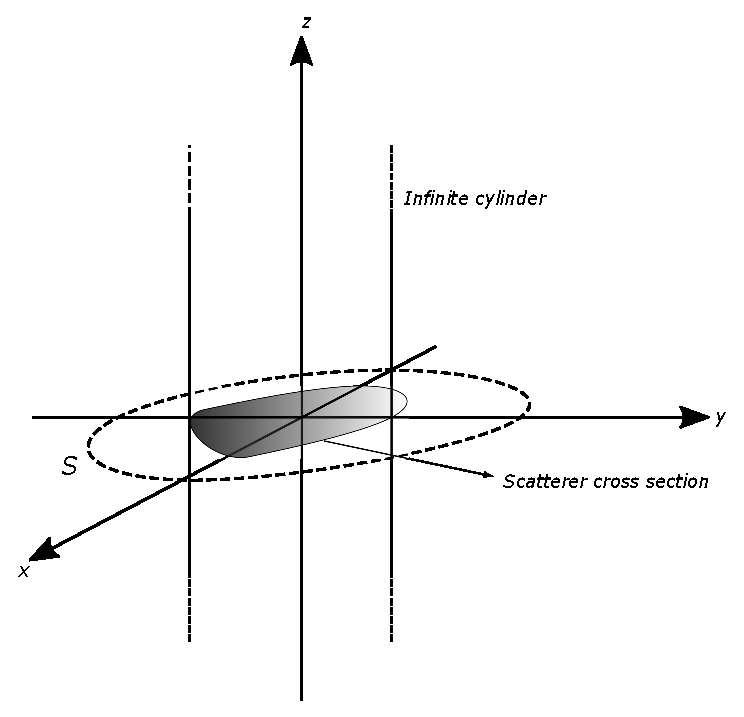
\includegraphics[width=0.4\textwidth]{./figuras/2dproblem}
				\caption{Infinite cylinder with inhomogeneous cross section.}
				\label{fig:2:2dproblem}
			\end{figure}
			\begin{eqnarray}
				E_{s_z}(\brho)\mathbf{z} &=& k_b^2 \int\limits_S\int_{-\infty}^{\infty}dz^\prime d\brhop\mathbf{\bar{G}}(\mathbf{r},\mathbf{r^\prime})\cdot\chi(\brhop)E_z(\brhop)\mathbf{z} \label{eq:2:2d:1} \\
				&=& k_b^2 \int\limits_S d\brhop \left[\int_{-\infty}^{\infty}dz^\prime\left(\mathbf{\bar{I}} + \frac{\nabla\nabla}{k_b^2}\right) \frac{-e^{jk_b|\mathbf{r}-\mathbf{r^\prime}|}}{4\pi|\mathbf{r}-\mathbf{r^\prime}|} \right]  \cdot\chi(\brhop)E_z(\brhop)\mathbf{z} \label{eq:2:2d:2}
			\end{eqnarray}
	
			%A integral em $z$ no lado direito da equação \eqref{eq:2:2d:2} tem resultado analítico conhecido \citep{balanis2012advanced}:
			The integral over $z$ on the right side of equation \eqref{eq:2:2d:2} is known \citep{balanis2012advanced}:
			\begin{equation}
				\int_{-\infty}^{\infty}dz^\prime\left(\mathbf{\bar{I}} + \frac{\nabla\nabla}{k_b^2}\right) \frac{e^{jk_b|\mathbf{r}-\mathbf{r^\prime}|}}{4\pi|\mathbf{r}-\mathbf{r^\prime}|}  = \frac{j}{4}H_0^{(2)}(k_b|\brho-\brhop|) \label{eq:2:2d:3}
			\end{equation}
		
			%\noindent onde $H_0^{(2)}$ é a função de Hankel de ordem zero e grau 2. Desta forma, \eqref{eq:2:2d:2} pode ser reescrita como:
			\noindent where $H_0^{(2)}$ is the Hankel function of the second kind. Thus, \eqref{eq:2:2d:2} can be rewritten as:
			\begin{equation}
				E_{s_z}(\brho) = -\frac{jk_b^2}{4} \int_S dS^\prime H_0^{(2)}(k_b|\brho-\brhop|) \chi(\brhop) E_z(\brhop)\label{eq:2:2d:4}
			\end{equation}
		
			%Similarmente, as equações \eqref{eq:2:waveequations:final}, \eqref{eq:2:eisp:5}, \eqref{eq:2:eisp:6} e \eqref{eq:2:eisp:9} podem ser reescritas como:
			Similarly, equations  \eqref{eq:2:waveequations:final}, \eqref{eq:2:eisp:5}, \eqref{eq:2:eisp:6}, and \eqref{eq:2:eisp:9} can be rewritten as:
			\begin{eqnarray}
				E_z(\brho) &=& E_{z_i}(\brho) - \frac{jk_b^2}{4} \int_S dS^\prime H_0^{(2)}(k_b|\brho-\brhop|) \chi(\brhop) E_z(\brhop) \label{eq:2:2d:5} \\
				E_{s_z}(\brho) &=& -\frac{jk_b^2}{4} \int_S dS^\prime H_0^{(2)}(k_b|\brho-\brhop|) J_{z_{eq}}(\brhop) \label{eq:2:2d:6} \\
				\chi(\brho)E_{z_i}(\brho) &=& J_{z_{eq}}(\brho) + \frac{jk_b^2}{4} \chi(\brho) \int_S dS^\prime H_0^{(2)}(k_b|\brho-\brhop|) J_{z_{eq}}(\brhop) \label{eq:2:2d:7} \\
				\beta(\brho)J_{z_{eq}}(\brho) &=& R(\brho)\beta(\brho)J_{z_{eq}}(\brho) \nonumber \\ && +~~ R(\brho)\left[ E_{z_i}(\brho) - \frac{jk_b^2}{4} \int_S dS^\prime H_0^{(2)}(k_b|\brho-\brhop|) J_{z_{eq}}(\brhop)\right] \label{eq:2:2d:8}
			\end{eqnarray}
		
			Recently, \cite{bevacqua2021effective} proposed to decompose the Hankel function in two terms using the known identity $H^{(2)}_0(x) = J_0(x) + Y_0$, where the $Y_0$ is the zero order Bessel function of second kind. Then, \eqref{eq:2:eisp:7} might be rewritten as:
			\begin{multline}
				\chi(\brho)E_{z_i}(\brho) = J_{z_{eq}}(\brho) + \frac{jk_b^2}{4} \chi(\brho) \int_S dS^\prime J_0(k_b|\brho-\brhop|) J_{z_{eq}}(\brhop) \\ + \frac{jk_b^2}{4} \chi(\brho) \int_S dS^\prime Y_0(k_b|\brho-\brhop|) J_{z_{eq}}(\brhop)  \label{eq:2:2d:greendecomp:csie}
			\end{multline}
		
			The first advantage in \eqref{eq:2:2d:greendecomp:csie} is that the first integral, which does not exhibit singularity, can be easily computed from the available scattered field data. Its meaning is the contribution of main spectral component of the radiating currents to the total field in $S$. The second advantage is the potential to mitigate the nonlinearity condition of the problem (see Subsection \ref{chap:problemstatement:eisp:4} for more information). The authors also provides a straightforward procedure to compute the first integral and a discretization formula to address the second integral.
		
		\subsection{Vector spaces and operator properties}\label{chap:problemstatement:eisp:3}
		
			%A função $\chi(\mathbf{r})$ é uma função contínua por partes, uma vez que representa as propriedades dielétricas dos meios no domínio. Desta forma, $\chi$ é uma função diferenciável e integrável exceto nas fronteiras dos meios. Já a função que representa o campo elétrico total, em problemas tridimensionais, pode apresentar descontinuidades em suas componentes devido à condições de interface entre os meios. No entanto, isso não acontece em problemas bidimensionais, uma vez que a componente $E_z$ é sempre perpendicular à normal definida na interface entre os meios. De qualquer maneira, essa grandeza é sempre integrável e diferenciável pelo menos no interior dos objetos. O mesmo vale para o campo espalhado. No entanto, ele é geralmente medido em meios homogêneos, ou seja, não costuma envolver discontinuidades.
			The $\chi(\mathbf{r})$ function is continuous by parts since it represents the dielectric properties of the media. Therefore, $\chi$ is an integrable and differentiable function except at the interface between media. The function which represents the total electric field, in three-dimensional problems, may have discontinuities in its components due to interface conditions. However, this does not happen in two-dimensional problems, since the $E_z$ component is always perpendicular to the normal defined on the interface between the media. Either way, the field is always integrable and differentiable. This is also true for the scattered field. However, it is generally measured in a homogeneous media, i.e., it does not usually involve discontinuities.
			
			%Levando em consideração a \eqref{eq:2:eisp:5}, o conjunto de todas campos espalhados pode ser definido em termos de um espaço linear de funções analíticas com crescimento exponencial no infinito e regular dentro de um subdomínio da região medição do campo $D$, o qual é exterior ao domínio do espalhador \citep{bucci1989degrees}. Essas funções são uniformemente limitadas nesse subdomínio uma vez que a corrente equivalente $\mathbf{J}_{eq}$ é uniformemente limitada. Em outras palavras, uma vez que o kernel de \eqref{eq:2:eisp:5} é analítico, este operador é compacto, e por isso, a imagem de qualquer conjunto limitado é pré-compacta \citep{bucci1989degrees}. Também é possível chegar às mesmas conclusões se, ao equiparmos os espaços de $\chi$ com a norma $L^{\infty}$ e o espaço de $\mathbf{E}$ com a norma $L^2$, assumirmos que o campo total dentro do espalhador é uniformemente limitado. Isto é coerente tendo em vista que o contraste e o campo incidente são limitados. Consequentemente, a corrente equivalente também pertence a um conjunto limitado e o campo espalhado pertence a um pré-compacto. Ademais, uma vez que o operador inverso de um compacto não pode ser contínuo, então o problema inverso é mal-posto.
			Taking into account \eqref{eq:2:eisp:5}, the set of all scattered fields can be defined in terms of a linear space of analytical functions with exponential growth at infinity and regular within a subdomain of the measurement region $D$, which is external to the scatterer domain \citep{bucci1989degrees}. These functions are uniformly bounded in this subdomain since the equivalent current $\mathbf{J}_{eq}$ is uniformly bounded. In other words, since the kernel of \eqref{eq:2:eisp:5} is analytical (except at singularities), this operator is compact, and therefore, the image of any bounded set is pre-compact \citep{bucci1989degrees}. It is also possible to reach the same conclusions if we assume that the total field within the scatterer is uniformly bounded, provided we equip the defined $\chi$ space with the $L^{\infty}$norm and the $\mathbf{E}$ space with the $L^2$ norm. This is consistent since the contrast and the incident field are limited. Consequently, the equivalent current also belongs to a bounded set and the scattered field belongs to a pre-compact one. Furthermore, since the inverse operator of a compact one cannot be continuous, then the inverse problem is ill-posed.
			
	%		%Portanto, podemos definir o espaço vetorial de funções de $\chi$ como um espaço de Hilbert $L^2(V)$ o qual é composto de funções que podem ser medidas e integráveis na definição de Lebesgue \citep{bartle1995elements}. No entanto, o espaço vetorial de  $\mathbf{E}(\mathbf{r})$ é mais restrito devido às equações de Maxwell \eqref{eq:2:maxwell:har:1}-\eqref{eq:2:maxwell:har:4}. Por isso, o espaço de $\mathbf{E}(\mathbf{r})$ e $\mathbf{E}_s(\mathbf{r})$ pode ser definido como um subconjunto $U\subset L^2(V)$.
	%		Thus, we can define the vector space of functions for $\chi$ as a Hilbert space $L^2(V)$ which is composed of functions that can be measured and integrable in the Lebesgue definition \citep{bartle1995elements}. However, the vector space of $\mathbf{E}(\mathbf{r})$ is more restricted due to Maxwell's equations \eqref{eq:2:maxwell:har:1}-\eqref{eq:2:maxwell:har:4}. Therefore, the space of $\mathbf{E}(\mathbf{r})$ and $\mathbf{E}_s(\mathbf{r})$ can be defined as a subset $U\subset L^2(V)$.
	%		
	%		%Se $\mathbf{E}$ fosse conhecido nas equações \eqref{eq:2:waveequations:final} e \eqref{eq:2:eisp:2}, os operadores $\mathcal{L}^D : L^2(V) \rightarrow U$ e $\mathcal{L}^S(V) : L^2 \rightarrow U$ seriam compactos e fracamente singulares, conforme o \autoref{the:app:functional:9}.
	%		If $\mathbf{E}$ were known in equations \eqref{eq:2:waveequations:final} and \eqref{eq:2:eisp:2}, the $\mathcal{L}^D : L^2(V) \rightarrow U$ and $\mathcal{L}^S(V) : L^2 \rightarrow U$ operators would be linear, compact, and weakly singular, according to \autoref{the:app:functional:9}.
		
		\subsection{Uniqueness, Stability and Nonlinearity}\label{chap:problemstatement:eisp:4}
			
			%Conforme discutido na \autoref{chap:problemstatement:inverse}, existem três critérios que precisam ser atendidos para que um problema seja considerado bem-posto. O problema inverso de espalhamento eletromagnético é mal-posto por não atender o critério de estabilidade. A condição de unicidade, embora garantida, é considerada apenas em análises teóricas do problema, i.e., em situações práticas, o problema não costuma ter solução única. Além disso, o problema é não-linear, o que confere outros aspectos ao problema.
			As discussed in Section \ref{chap:problemstatement:inverse}, three criteria need to be satisfied for a problem to be considered well-posed. EISP is ill-posed because it does not meet the stability criterion. The condition of uniqueness is considered only in some theoretical analyzes, i.e., in practical situations, the problem does not usually have a single solution. In addition, the problem is non-linear, which provides other aspects to the problem.
			
			%Uma vez que se trata de um problema físico com modelagem matemática coerente, a condição de existência de solução não é questionada. De um ponto de vista teórico, é mais importante questionar se o problema tem solução única. Conforme demonstrado por \cite{colton1992uniqueness}, a unicidade da permissividade relativa para um dado padrão de campo distante é garantida sob certas condições, dentre elas: um número fixo de número de onda, todas as direções de incidência e todas as polarizações do campo incidente. Todavia, em situações práticas, todas essas informações nem sempre estão disponíveis. Vale à pena destacar também que existem situações para as quais a unicidade não é garantida do ponto de vista analítico, como por exemplo, em problemas nos quais a permissividade e permeabilidade podem ser zero ou infinito.
			As demonstrated by \cite{colton1992uniqueness}, the uniqueness of the relative permittivity for a given distant field pattern is guaranteed under certain conditions, among them: a fixed number of wavenumber, all directions of incidence, and all polarizations of the field incident. Therefore, the existence condition is also fulfilled. However, in practical situations, all of this information is not always available. It is also worth noting that there are situations for which uniqueness is not guaranteed from an analytical point of view, such as, problems in which permittivity and permeability can be zero or infinite.
			
			%Mesmo que uma quantidade suficiente de informação esteja disponível para que o problema tenha solução única, a relação entre as variáveis conhecidas e desconhecidas não é contínua \citep{chen2017}. Conforme já foi demonstrado na literatura \citep{stefanov1990stability,caro2010stable}, para um problema envolvendo espalhadores dielétricos, se o erro nos dados conhecidos são no máximo $\delta$, então o pior cenário do erro na solução é da ordem de $\ln|\delta|^{-s}$, onde $0<s<1$. Isto é conhecido como uma estimativa de estabilidade do problema e, quando $\delta\rightarrow0$, pela regra de L'Hôpital, a ordem do erro aumenta drasticamente. Esse tipo de situação é conhecido na literatura como problema exponencialmente ou severamente mal-posto. Esse tipo de condição não pode ser mudada se tivermos infinitas medições de campo. No entanto, a estabilidade pode ser aumentada com algumas estratégias, como por exemplo, o aumento de frequências de operação \citep{bao2015inverse,nagayasu2013increasing,isakov2016increasing}.
			Even if a sufficient amount of information is available for uniqueness, the relationship between known and unknown variables is not continuous \citep{chen2017}. As already demonstrated in the literature \citep{stefanov1990stability,caro2010stable}, for a problem involving dielectric scatterers, if the error in the known data is at most $\delta$, then the worst scenario of the error in the solution is in the order of $\ln|\delta|^{-s}$, where $0<s<1$. This is known as a problem stability estimate and, when $\delta\rightarrow0$, by the L'Hôpital rule, the error order increases dramatically. This type of situation is known in the literature as an exponential or severely ill-posed problem. This type of condition cannot change if we have infinite field measurements. However, stability can increase with some strategies, such as, for example, increasing operating frequencies \citep{bao2015inverse,nagayasu2013increasing,isakov2016increasing}.
			
			%Conforme dito anteriormente, a relação entre contraste e campo espalhado não é linear uma vez que existem interações mútuas entre correntes induzidas. Por isso, o campo não pode ser interpretado como uma superposição linear de respostas individuais. Além disso, a não-linearidade do problema não é do tipo convexa, ou seja, do ponto de vista de otimização, podem haver múltiplos mínimos locais os quais podem fazer com que algoritmos fiquem presos em soluções falsas \citep{chen2017,bucci1997electromagnetic}. Por isso, encontrar a solução exata para o problema se torna mais complicado.
			As stated earlier, the relationship between contrast and scattered field is not linear since there are mutual interactions between induced currents. Therefore, we cannot interpret the field as a linear superposition of individual responses. Besides, the nonlinearity of the problem is not of the convex kind, i.e., from the optimization point of view, there may be multiple local minima which can cause algorithms to get trapped in false solutions \citep{chen2017,bucci1997electromagnetic}. Therefore, finding the exact solution becomes more complex. 
			
			A deeper explanation on non-linearity is found in \cite{bucci2001degree}. The authors developed the Degree of Nonlinearity (DNL) which is indicator to how difficult is solving the correspond EISP. Considering the state equation in the operator \eqref{eq:2:eisp:4}, the total field $E_z$ may be rewritten as:
			\begin{equation}
				\mathbf{E}_z(\mathbf{r}) = \left(\mathcal{I} - \mathcal{L}^S\{\chi(\mathbf{r})\}\right)^{-1} \mathbf{E}_i(\mathbf{r})
			\end{equation}
		
			\noindent where $\mathcal{I}$ is the identity operator and $$\mathcal{L}^S\{\chi(\mathbf{r})\} = - k_b^2\int_V d\mathbf{r^\prime} \mathbf{\bar{G}}(\mathbf{r},\mathbf{r^\prime})\cdot\chi(\mathbf{r^\prime}).$$
			
			When the $L^2$-norm over $ \mathcal{L}^S\{\chi(\mathbf{r})\}$ is lower than 1, the inverse operator is approximated by Neumann series, i.e.:
			\begin{equation}
				\left(\mathcal{I} - \mathcal{L}^S\{\chi(\mathbf{r})\}\right)^{-1} = \mathcal{I} + \mathcal{L}^S\{\chi(\mathbf{r})\} + \left(\mathcal{L}^S\{\chi(\mathbf{r})\}\right)^2 + \cdots + \left(\mathcal{L}^S\{\chi(\mathbf{r})\}\right)^n + \cdots
			\end{equation}
			
			Then, \cite{bucci2001degree} defined DNL indicator as $||\mathcal{L}^S\{\chi(\mathbf{r})\}||_{L^2}$. They observed that, the smaller than 1 DNL is, the stronger linear approximation is. As DNL tends to 1, a polynomial relation holds true between data and unknowns. The larger the order of polynomial is, the larger the number of local minima. When DNL is greater than 1, then a non-polynomial relation holds true. Therefore, the larger the DNL, the larger overall difficulty of the problem due its nonlinearity. In these cases, the possible number of local minima in respect to some cost functional can be higher, which increases the difficulty of finding the global minimum that defines the solution of the inverse problem. Moreover, the indicator is also applied to the two-dimensional case \eqref{eq:2:2d:5}, the Contrast Source Integral Equation \eqref{eq:2:2d:7}, its Extended-Born version \eqref{eq:2:2d:8}, and when the Green's function is decomposed \citep{durso2010solution,bevacqua2021effective}. In \cite{durso2010solution}, the authors provide criteria for choosing between \eqref{eq:2:2d:7} and \eqref{eq:2:2d:8}. In \cite{bevacqua2021effective}, the authors show that the Green's Function Decomposition formulation has a much lower growth of DNL than the traditional Contrast Source Integral \eqref{eq:2:2d:7} when the scatterer size increases. \cite{bevacqua2021quantitative} showed that, for certain configurations of scatterers and values of $\beta$ in \eqref{eq:2:eisp:9}, the DNL can be drastically reduced (mainly when $\beta\ge2$). The authors also showed significant reductions in the degree of non-linearity when the Y0 \eqref{eq:2:2d:greendecomp:csie} and NIE \eqref{eq:2:eisp:9} formulations are combined \citep{bevacqua2021new}. For $\beta=6$, the results showed less DNL growth as the scatterer grew when compared to the other formulations.
			
			%Os autores mostraram que, para determinadas configurações de espalhadores e valores de $\beta$ em \eqref{eq:2:eisp:9}, o DNL pode ser reduzido drasticamente (principalmente quando $\beta\ge2$). Os autores também mostraram significativas reduções do grau de não-linearidade quando a formulações Y0 \eqref{eq:2:2d:greendecomp:csie} e NIE \eqref{eq:2:eisp:9} são combinadas. Para $\beta=6$, os resutados mostraram um crescimento menor do DNL conforme o espalhador crescia em comparação com as outras formulações.
			
		\subsection{Degrees of Freedom}\label{chap:problemstatement:eisp:5}
	
			%Do ponto de vista analítico, dois campos são distinguíveis quando suas definições são distintas entre si. No entanto, quando essas grandezas físicas diferem muito pouco entre si, elas podem ser indistinguíveis na prática. Existem muitos fatores que podem contribuir para a impossibilidade de destinguir campos, como por exemplo, ruídos, dinâmicas dos mecanismos de medição, precisão e erros numérios. Baseado na definição do conceito de distinção é que é possível definir diferentes estados do sistemas, e com isso, a noção de um número mínimo de parâmetros independentes que podem descrever o sistema até uma certa precisão. Este assunto tem um papel importante em EISPs uma vez que campos espalhados que sejam considerados indistinguíveis vão ter reconstruções idênticas as quais nem sempre vão representar bem os meios investigados.
			From an analytical point of view, two fields are distinguishable when their definitions are distinct from each other. However, when these physical quantities differ very little from each other, they can be indistinguishable in practice. Many factors can contribute to the impossibility of distinguishing fields, such as, for example, noise, dynamics of measurement mechanisms, precision, and numerical errors. Based on the definition of the concept of distinction, it is possible to define different states of the system, and with that, the notion of a minimum number of independent parameters that can describe the system to a certain precision. This issue plays an important role in EISPs since scattered fields that are considered indistinguishable will have identical reconstructions which will not always represent the investigated media well.
			
			%No primeiro trabalho sobre o tema, \cite{bucci1989degrees} mostraram que o número de graus de liberdade de um campo espalhado é essencialmente igual ao número de Nyquist definido proporcionalmente às dimensões das regiões de fonte e de observação. Particularmente, o número de Nyquist $N_0$ foi definido como:
			In the first work on the subject, \cite{bucci1989degrees} showed that the number of Degrees of Freedom (DoF) in a scattered field is essentially equal to the Nyquist number defined in proportion to the dimensions of the source and observation regions. In particular, the Nyquist $N_0$ number was defined as:
			\begin{equation}
				N_0 = \frac{2SW_0}{\pi} \approx \frac{2Ska}{\pi} \label{eq:2:dof:1}
			\end{equation}
		
			%\noindent onde $S$ é a metade do comprimento do domínio de observação, $W_0$ é a largura de banda do sinal, $k_b$ é o número de onda do meio de fundo e $a$ é o raio máximo do domínio que os espalhadores ocupam. Este, então, seria o número mínimo de parâmetros (informação) necessário para representar com uma certa precisão o campo espalhado. Os autores também concluíram uma interpolação amostral em pontos equidistantes seria uma reconstrução praticamente ótima do campo espalhado.
			\noindent where $S$ is half the length of the observation domain, $W_0$ is the signal bandwidth, $k$ is the source wavenumber  and $a$ is the maximum radius of the domain that the scatterers occupy. This, then, would be the minimum number of parameters (information) necessary to represent the spread field with a certain precision. The authors also concluded that a sample interpolation at equidistant points would be a practically optimal reconstruction of the scattered field.
			
			%Posteriormente, \cite{bucci1997electromagnetic}, baseados no fato de que apenas representação de dimensão finita do contraste pode ser reconstruída, avaliaram qual a dimensão do espaço de dados coerente com uma certa configuração do espaço que representa o contraste. Esta avaliação foi feita tanto para um caso de única indicidência como múltiplas. No caso de incidência simples, os autores perceberam que a relação entre quantidade e valor de autovalores do kernel em \eqref{eq:2:eisp:5} tem um comportamento semelhante à função degrau, i.e., a medida que a quantidade de autovalores cresce, seus valores sofrem uma queda brusca a partir de um certo limiar. Além disso, quando maior o espalhador, mais brusca a queda. Esse comportamento também em relação ao erro de aproximação, o que significa dizer que o número dos graus de liberdade pode ser identificado uma quantidade de autovalores para o qual o erro de aproximação ultrapassa um certo limiar estabelecido. Para o caso de fontes esféricas e superfícies de observação esféricas e concêntricas, se $k_ba \gg 1$, então o número de graus de liberdade $M$ será:
			Subsequently, \cite{bucci1997electromagnetic} evaluated the dimension of the data space which is consistent with a certain contrast space configuration. Their analysis is based on the fact that only a finite-dimensional representation of the contrast can be reconstructed. This assessment was made for both single and multiple cases. In the case of simple incidence, the authors realized that the relationship between amount and value of kernel eigenvalues in \eqref{eq:2:eisp:5} behaves similarly to the step function, i.e., as the number of eigenvalues grows, their values fall sharply from a certain threshold. Also, the larger the scatterer, the more sudden the fall. This behavior is also observed when we consider the approximation error, which allows us to identify the number of degrees of freedom by the number of eigenvalues for which the approximation error exceeds a certain established threshold. For spherical sources and spherical (concentric) observation surfaces, if $k_ba \gg 1$, then DoF is approximated by:
			\begin{equation}
				DoF \approx (ka)^2 \label{eq:2:dof:2}
			\end{equation}
		
			%Num caso bidimensional de círculos concêntricos para fontes circulares:
			In a two-dimensional case of concentric circles for circular sources:
			\begin{equation}
				DoF \approx 2ka \label{eq:2:dof:3}
			\end{equation}
		
			%Já no caso da incidência múltipla, os autores afirmaram que o número de parâmetros independentes não pode ser maior que $M^2/2$, onde $M$ é o número de graus de liberdade para incidência simples. Em seus experimentos, os autores não visualizaram diferença significativa entre uma amostragem $32\times32$ e uma $36\times36$ no caso de um objeto circular de baixo contraste com diâmetro $5\lambda_b$ ($M\approx32$).
			Considering multiple incidences, the authors stated that the number of independent parameters must not be greater than $DoF^2/2$, where $DoF$ is the number of degrees of freedom for simple incidence. In their experiments, the authors did not observe a significant difference between a $32\times32$ and a $36\times36$ scattered matrices, considering a low contrast circular object with a diameter of $5\lambda_b$ ($DoF\approx32$).
			
			 \cite{chew1994inverse} also discussed this issue. Firstly, they demonstrated why solving \eqref{eq:2:eisp:5} for $\mathbf{J}_{eq}$ and evaluating $\mathbf{E}$ and $\chi$ through \eqref{eq:2:waveequations:final} and $\mathbf{J}_{eq}/\mathbf{E}$, respectively, is not an adequate approach. Although it seems attractive since there is no iteration process, the solution in practical situations is not unique, as discussed in Subsection \ref{chap:problemstatement:eisp:4}. One of the solutions is due to non-radiating sources which are also inverse solutions to the Green's function. The non-radiating solution is due to the non-trivial null space in \eqref{eq:2:eisp:5}, i.e., there is a non-trivial solution for $\mathbf{E}_s=\mathbf{0}$. Consequently, if a unique solution to \eqref{eq:2:eisp:5} is obtained (e.g., minimum norm solution through pseudo-inverse method \citep{ney1984solution}), the null space solution is eliminated. Even though, it does not contribute to the scattered field, it does contribute to the total field within the scatterer. Therefore, without the null space solution, the total field obtained by the application of $\chi\mathbf{E}=\mathbf{J}_{eq}$ in \eqref{eq:2:waveequations:final} and the following contrast function estimation by $\mathbf{J}_{eq}/\mathbf{E}$ will not be correct.
			
			Second, the authors stated that a very large number of measurements will not make the null space smaller, which agrees with \cite{bucci1989degrees} and  \cite{bucci1997electromagnetic}. In addition, the difference in the dimensionality between the measurement and image domains is also a practical obstacle for raising the number of measurements. The authors called the growth of linear dependency as the number of measurements increases as the \textit{law of diminishing return}. Their explanation is based on the high-spatial-components of the induced current which generates evanescent waves that decay fast away from the scatterer and are very small at the measurement space. The decay is also related to the nature of the Green's function which can be compared to a low-pass filter. These components also contributes to the null space. Through the Fourier analysis of the scattered field, the authors came to the same conclusion as \cite{bucci1989degrees} about the Nyquist number as upper bound of sampling rate.
			
			Finally, some efforts have been made towards a numerical approach for computing DoF. \cite{lin2021study} proposed to modify the Green function taking into account the maximum contrast value and evaluate DoF based on the singular values of the Green function. When the maximum contrast is not available, then it is assumed that the contrast tends to infinity and a new modification for the Green function is formulated. 
		
	\section{Conclusion}
	
		%Este capítulo apresentou uma breve discussão sobre os aspectos teóricos do problema inverso de espalhamento eletromagnético. A seção 1 introduziu as grandezas e suas relações mais básicas levando em consideração um modelo com meios lineares, isotrópicos, não-dispersivos e não-magnéticos. A seção 2 apresentou o desenvolvimento da equação integral \eqref{eq:2:waveequations:final} que é a base para o problema. Baseado na definição proposta por \cite{hadamard1923lectures}, a seção 3 discutiu o que é um problema inverso mal-posto através dos critérios de existência, unicidade e estabilidade de solução. Além disso, a seção também apresentou a formulação geral de operadores de regularização através da equação \eqref{eq:2:inverse:2}. A seção 4 definiu o problema inverso de espalhamento eletromagnético apresentando as formulações tridimensionais através das equações \eqref{eq:2:eisp:2}, \eqref{eq:2:eisp:5}-\eqref{eq:2:eisp:9}; e as formulações bidimensionais baseadas no Modo Transversal Magnético em $z$ descritas nas equações \eqref{eq:2:2d:4}-\eqref{eq:2:2d:8}. Além disso, foram discutidas as propriedades dos espaços vetorais e operadores envolvidos no problema. Também foi demonstrado que o problema pode ter solução única em algumas situações que dificilmente são possíveis na prática. De qualquer maneira, até quando existe solução única, o problema é mal-posto por questões de instabilidade cuja a explicação pode ser demonstrada através da teoria de operadores inversos de operadores compactos. Ademais, a instabilidade pode ser quantificada através da estimativa de pior-caso a qual é exponencial para o problema. Além destes fatores que dificultam a solução do problema, a não-linearidade do tipo não-convexo é uma característica importante a qual pode fazer com que algoritmos de otimização fiquem presos em mínimos locais que representam imagens espúrias. Por fim, os graus de liberdade do problema foram definidos através da \eqref{eq:2:dof:3} o qual é uma medida importante para a determinação da quantidade necessária de observações do campo espalhado considerando uma determinada configuração do problema.
		This chapter presented a brief discussion of the theoretical aspects of EISP. Section \ref{chap:problemstatement:eletromagnetic} introduced the physical quantities and their most basic relations taking into account a model with linear, isotropic, non-dispersive, and non-magnetic materials. Section \ref{chap:problemstatement:integral} presented the development of the integral equation \eqref{eq:2:waveequations:final} that is the basis for the problem.
		
		Based on the definition proposed by \cite{hadamard1923lectures}, Section \ref{chap:problemstatement:inverse} discussed what is an an ill-posed inverse problem through the criteria of existence, uniqueness, and stability of the solution. The section also presented the general formulation of regularization operators using equation \eqref{eq:2:inverse:2}.
		
		Section \ref{chap:problemstatement:eisp} defined the electromagnetic inverse scattering problem by presenting three-dimensional formulations through equations \eqref{eq:2:eisp:2}, \eqref{eq:2:eisp:5}-\eqref{eq:2:eisp:9}; and the two-dimensional formulations based on the TMz mode described through equations \eqref{eq:2:2d:4}-\eqref{eq:2:2d:8}. Besides, the properties of the vector spaces and operators were discussed. It has also been shown that the problem can have a unique solution in some situations which are hardly possible in practice. Nevertheless, even when there is a unique solution, the problem is still ill-posed for reasons of instability whose explanation can be demonstrated through the theory of inverse operators of compact ones. Furthermore, instability can be quantified through the worst-case estimate which is exponential for the problem. In addition to these factors that contribute to the complexness of the problem, non-convex non-linearity is an important feature that can cause optimization algorithms to be trapped in local minima which may represent spurious images. Finally, the degrees of freedom of the problem were defined using \eqref{eq:2:dof:3}, which is an important measure for determining the necessary amount of observations of the scattered field considering a given configuration of the problem.
		